%%%%%%%%%%%%%%%%%%%%%%%%%%%%%%%%%%%%%%%%%%%%%%%%%
% Chapter: Job Allocation Management
%%%%%%%%%%%%%%%%%%%%%%%%%%%%%%%%%%%%%%%%%%%%%%%%%
\chapter{Job Management and Reporting}
\label{chap:api_job_mgmt}

The job management \acp{API} provide an application with the ability to orchestrate its operation in partnership with the \ac{SMS}.
Members of this category include the \refapi{PMIx_Allocation_request_nb}, \refapi{PMIx_Job_control_nb}, and \refapi{PMIx_Process_monitor_nb} \acp{API}.

%%%%%%%%%%%%%%%%%%%%%%%%%%%%%%%%%%%%%%%%%%%%%%
%%%%%%%%%%%%%%%%%%%%%%%%%%%%%%%%%%%%%%%%%%%%%%
\section{Query}
\label{chap:api_proc_mgmt:query}

As the level of interaction between applications and the host \ac{SMS} grows, so too does the need for the application to query the \ac{SMS} regarding its capabilities and state information. \ac{PMIx} provides a generalized query interface for this purpose, along with a set of standardized attribute keys to support a range of requests. This includes requests to determine the status of scheduling queues and active allocations, the scope of \ac{API} and attribute support offered by the \ac{SMS}, namespaces of active jobs, location and information about a job's processes, and information regarding available resources.

An example use-case for the \refapi{PMIx_Query_info_nb} \ac{API} is to ensure clean job completion. Time-shared systems frequently impose maximum run times when assigning jobs to resource allocations. To shut down gracefully, e.g., to write a checkpoint before termination, it is necessary for an application to periodically query the resource manager for the time remaining in its allocation. This is especially true on systems for which allocation times may be shortened or lengthened from the original time limit. Many resource managers provide \acp{API} to dynamically obtain this information, but each \ac{API} is specific to the resource manager.

\ac{PMIx} supports this use-case by defining an attribute key (\refattr{PMIX_TIME_REMAINING}) that can be used with the \refapi{PMIx_Query_info_nb} interface to obtain the number of seconds remaining in the current job allocation. Note that one could alternatively use the \refapi{PMIx_Register_event_handler} \ac{API} to register for an event indicating incipient job termination, and then use the \refapi{PMIx_Job_control_nb} \ac{API} to request that the host \ac{SMS} generate an event a specified amount of time prior to reaching the maximum run time. \ac{PMIx} provides such alternate methods as a means of maximizing the probability of a host system supporting at least one method by which the application can obtain the desired service.

The following \acp{API} support query of various session and environment values.

%%%%%%%%%%%
\subsection{\code{PMIx_Resolve_peers}}
\declareapi{PMIx_Resolve_peers}

%%%%
\summary

Obtain the array of processes within the specified namespace that are executing on a given node.

%%%%
\format

\versionMarker{1.0}
\cspecificstart
\begin{codepar}
pmix_status_t
PMIx_Resolve_peers(const char *nodename,
                   const pmix_nspace_t nspace,
                   pmix_proc_t **procs, size_t *nprocs)
\end{codepar}
\cspecificend

\begin{arglist}
\argin{nodename}{Name of the node to query (string)}
\argin{nspace}{namespace (string)}
\argout{procs}{Array of process structures (array of handles)}
\argout{nprocs}{Number of elements in the \refarg{procs} array (integer)}
\end{arglist}

Returns \refconst{PMIX_SUCCESS} or a negative value corresponding to a PMIx error constant.

%%%%
\descr

Given a \refarg{nodename}, return the array of processes within the specified \refarg{nspace}
that are executing on that node.
If the \refarg{nspace} is \code{NULL}, then all processes on the node will be returned.
If the specified node does not currently host any processes, then the returned array will be \code{NULL}, and \refarg{nprocs} will be \code{0}.
The caller is responsible for releasing the \refarg{procs} array when done with it.
The \refmacro{PMIX_PROC_FREE} macro is provided for this purpose.

%%%%%%%%%%%
\subsection{\code{PMIx_Resolve_nodes}}
\declareapi{PMIx_Resolve_nodes}

%%%%
\summary

Return a list of nodes hosting processes within the given namespace.

%%%%
\format

\versionMarker{1.0}
\cspecificstart
\begin{codepar}
pmix_status_t
PMIx_Resolve_nodes(const char *nspace, char **nodelist)
\end{codepar}
\cspecificend

\begin{arglist}
\argin{nspace}{Namespace (string)}
\argout{nodelist}{Comma-delimited list of nodenames (string)}
\end{arglist}

Returns \refconst{PMIX_SUCCESS} or a negative value corresponding to a PMIx error constant.

%%%%
\descr

Given a \refarg{nspace}, return the list of nodes hosting processes within that namespace.
The returned string will contain a comma-delimited list of nodenames.
The caller is responsible for releasing the string when done with it.


%%%%%%%%%%%
\subsection{\code{PMIx_Query_info_nb}}
\declareapi{PMIx_Query_info_nb}

%%%%
\summary

Query information about the system in general.

%%%%
\format

\versionMarker{2.0}
\cspecificstart
\begin{codepar}
pmix_status_t
PMIx_Query_info_nb(pmix_query_t queries[], size_t nqueries,
                   pmix_info_cbfunc_t cbfunc, void *cbdata)
\end{codepar}
\cspecificend

\begin{arglist}
\argin{queries}{Array of query structures (array of handles)}
\argin{nqueries}{Number of elements in the \refarg{queries} array (integer)}
\argin{cbfunc}{Callback function \refapi{pmix_info_cbfunc_t} (function reference)}
\argin{cbdata}{Data to be passed to the callback function (memory reference)}
\end{arglist}

Returns one of the following:

\begin{itemize}
\item \refconst{PMIX_SUCCESS} indicating that the request has been accepted for processing and the provided callback function will be executed upon completion of the operation. Note that the library must not invoke the callback function prior to returning from the \ac{API}.
\item a non-zero \ac{PMIx} error constant indicating a reason for the request to have been rejected. In this case, the provided callback function will not be executed
\end{itemize}

If executed, the status returned in the provided callback function will be one of the following constants:

\begin{itemize}
\item \refconst{PMIX_SUCCESS} All data has been returned
\item \refconst{PMIX_ERR_NOT_FOUND} None of the requested data was available
\item \refconst{PMIX_ERR_PARTIAL_SUCCESS} Some of the data has been returned
\item \refconst{PMIX_ERR_NOT_SUPPORTED} The host \ac{RM} does not support this function
\item a non-zero \ac{PMIx} error constant indicating a reason for the request's failure
\end{itemize}

\reqattrstart
\ac{PMIx} libraries that support this \ac{API} are required to support the following attributes:

\pastePRIAttributeItem{PMIX_QUERY_REFRESH_CACHE}
\pastePRIAttributeItem{PMIX_SESSION_INFO}
\pastePRIAttributeItem{PMIX_JOB_INFO}
\pastePRIAttributeItem{PMIX_APP_INFO}
\pastePRIAttributeItem{PMIX_NODE_INFO}
\pastePRIAttributeItemBegin{PMIX_PROCID} Specifies the process ID whose information is being requested - e.g., a query asking for the \refattr{PMIX_LOCAL_RANK} of a specified process. Only required when the request is for information on a specific process.
\pastePRIAttributeItemEnd
\pastePRIAttributeItemBegin{PMIX_NSPACE} Specifies the namespace of the process whose information is being requested - e.g., a query asking for the \refattr{PMIX_LOCAL_RANK} of a specified process. Must be accompanied by the \refattr{PMIX_RANK} attribute. Only required when the request is for information on a specific process.
\pastePRIAttributeItemEnd
\pastePRIAttributeItemBegin{PMIX_RANK} Specifies the rank of the process whose information is being requested - e.g., a query asking for the \refattr{PMIX_LOCAL_RANK} of a specified process. Must be accompanied by the \refattr{PMIX_NSPACE} attribute. Only required when the request is for information on a specific process.
\pastePRIAttributeItemEnd
\pastePRIAttributeItem{PMIX_QUERY_ATTRIBUTE_SUPPORT}
\pastePRIAttributeItem{PMIX_CLIENT_ATTRIBUTES}
\pastePRIAttributeItem{PMIX_SERVER_ATTRIBUTES}
\pastePRIAttributeItem{PMIX_HOST_ATTRIBUTES}
\pastePRIAttributeItem{PMIX_TOOL_ATTRIBUTES}

Note that inclusion of the \refattr{PMIX_PROCID} directive and either the \refattr{PMIX_NSPACE} or the \refattr{PMIX_RANK} attribute will return a \refconst{PMIX_ERR_BAD_PARAM} result, and that the inclusion of a process identifier must apply to all keys in that \refstruct{pmix_query_t}. Queries for information on multiple specific processes therefore requires submitting multiple \refstruct{pmix_query_t} structures, each referencing one process.

\ac{PMIx} libraries are not required to directly support any other attributes for this function. However, any provided attributes must be passed to the host \ac{SMS} daemon for processing, and the \ac{PMIx} library is \textit{required} to add the \refPRIAttributeItem{PMIX_USERID} and the \refPRIAttributeItem{PMIX_GRPID} attributes of the client process making the request.

\divider

Host environments that support this operation are required to support the following attributes as qualifiers to the request:

\pastePRRTEAttributeItemBegin{PMIX_PROCID} Specifies the process ID whose information is being requested - e.g., a query asking for the \refattr{PMIX_LOCAL_RANK} of a specified process. Only required when the request is for information on a specific process.
\pastePRIAttributeItemEnd

\pastePRRTEAttributeItemBegin{PMIX_NSPACE} Specifies the namespace of the process whose information is being requested - e.g., a query asking for the \refattr{PMIX_LOCAL_RANK} of a specified process. Must be accompanied by the \refattr{PMIX_RANK} attribute. Only required when the request is for information on a specific process.
\pastePRIAttributeItemEnd

\pastePRRTEAttributeItemBegin{PMIX_RANK} Specifies the rank of the process whose information is being requested - e.g., a query asking for the \refattr{PMIX_LOCAL_RANK} of a specified process. Must be accompanied by the \refattr{PMIX_NSPACE} attribute. Only required when the request is for information on a specific process.
\pastePRIAttributeItemEnd

Note that inclusion of the \refattr{PMIX_PROCID} directive and either the \refattr{PMIX_NSPACE} or the \refattr{PMIX_RANK} attribute will return a \refconst{PMIX_ERR_BAD_PARAM} result, and that the inclusion of a process identifier must apply to all keys in that \refstruct{pmix_query_t}. Queries for information on multiple specific processes therefore requires submitting multiple \refstruct{pmix_query_t} structures, each referencing one process.

\optattrstart
The following attributes are optional for host environments that support this operation:

\pastePRRTEAttributeItem{PMIX_QUERY_NAMESPACES}
\pastePRRTEAttributeItem{PMIX_QUERY_JOB_STATUS}
\pasteAttributeItem{PMIX_QUERY_QUEUE_LIST}
\pasteAttributeItem{PMIX_QUERY_QUEUE_STATUS}
\pastePRRTEAttributeItem{PMIX_QUERY_PROC_TABLE}
\pastePRRTEAttributeItem{PMIX_QUERY_LOCAL_PROC_TABLE}
\pastePRRTEAttributeItem{PMIX_QUERY_SPAWN_SUPPORT}
\pastePRRTEAttributeItem{PMIX_QUERY_DEBUG_SUPPORT}
\pastePRRTEAttributeItem{PMIX_QUERY_MEMORY_USAGE}
\pastePRRTEAttributeItem{PMIX_QUERY_REPORT_AVG}
\pastePRRTEAttributeItem{PMIX_QUERY_REPORT_MINMAX}
\pasteAttributeItem{PMIX_QUERY_ALLOC_STATUS}
\pastePRRTEAttributeItem{PMIX_TIME_REMAINING}
\pastePRRTEAttributeItemBegin{PMIX_SERVER_URI} Requests the URI of the specified \ac{PMIx} server's \ac{PMIx} connection. Defaults to requesting the information for the local \ac{PMIx} server.
\pastePRRTEAttributeItemEnd
\pastePRRTEAttributeItemBegin{PMIX_PROC_URI} Requests the URI of the specified \ac{PMIx} server's out-of-band connection. Defaults to requesting the information for the local \ac{PMIx} server.
\pastePRRTEAttributeItemEnd

\optattrend

%%%%
\descr

Query information about the system in general.
This can include a list of active namespaces, network topology, etc.
Also can be used to query node-specific info such as the list of peers executing on a given node.
We assume that the host \ac{RM} will exercise appropriate access control on the information.

NOTE: There is no blocking form of this API as the structures passed to query info differ from those for receiving the results.

The \refarg{status} argument to the callback function indicates if requested data was found or not.
An array of \refstruct{pmix_info_t} will contain each key that was provided and the corresponding value that was found. Requests for keys that are not found will return the key paired with a value of type \refconst{PMIX_UNDEF}.

\adviceimplstart
Information returned from \refapi{PMIx_Query_info_nb} shall be locally cached so that retrieval by subsequent calls to \refapi{PMIx_Get} or \refapi{PMIx_Query_info_nb} can succeed with minimal overhead. The local cache shall be checked prior to querying the \ac{PMIx} server and/or the host environment. Queries that include the \refattr{PMIX_QUERY_REFRESH_CACHE} attribute shall bypass the local cache and retrieve a new value for the query, refreshing the values in the cache upon return.
\adviceimplend

\subsubsection{Using \refapi{PMIx_Get} vs \refapi{PMIx_Query_info_nb}}
\label{chap:api_job_mgmt:query}

Both \refapi{PMIx_Get} and \refapi{PMIx_Query_info_nb} can be used to retrieve information about the system. In general, the \emph{get} operation should be used to retrieve:

\begin{itemize}
\item information provided by the host environment at time of job start. This includes information on the number of processes in the job, their location, and possibly their communication endpoints
\item information posted by processes via the \refapi{PMIx_Put} function
\end{itemize}

This information is largely considered to be \emph{static}, although this will not necessarily be true for environments supporting dynamic programming models or fault tolerance. Note that the \refapi{PMIx_Get} function only accesses information about execution environments - i.e., its scope is limited to values pertaining to a specific \refterm{session}, \refterm{job}, \refterm{application}, process, or node. It cannot be used to obtain information about areas such as the status of queues in the \ac{WLM}.

In contrast, the \emph{query} option should be used to access:

\begin{itemize}
\item system-level information (such as the available \ac{WLM} queues) that would generally not be included in job-level information provided at job start
\item dynamic information such as application and queue status, and resource utilization statistics. Note that the \refattr{PMIX_QUERY_REFRESH_CACHE} attribute must be provided on each query to ensure current data is returned
\item information created post job start, such as process tables
\item information requiring more complex search criteria than supported by the simpler \refapi{PMIx_Get} \ac{API}
\item queries focused on retrieving multi-attribute blocks of data with a single request, thus bypassing the single-key limitation of the \refapi{PMIx_Get} \ac{API}
\end{itemize}

In theory, all information can be accessed via \refapi{PMIx_Query_info_nb} as the local cache is typically the same datastore searched by \refapi{PMIx_Get}. However, in practice, the overhead associated with the \emph{query} operation may (depending upon implementation) be higher than the simpler \emph{get} operation due to the need to construct and process the more complex \refstruct{pmix_query_t} structure. Thus, requests for a single key value are likely to be accomplished faster with \refapi{PMIx_Get} versus the \emph{query} operation.

\subsubsection{Accessing attribute support information}
\label{chap:api_job_mgmt:queryattrs}

Information as to attributes supported by either the \ac{PMIx} implementation or its host environment can be obtained via the \refapi{PMIx_Query_info_nb} \ac{API}. The \refattr{PMIX_QUERY_ATTRIBUTE_SUPPORT} attribute must be listed as the first entry in the \refarg{keys} field of the \refstruct{pmix_query_t} structure, followed by the name of the function whose attribute support is being requested - support for multiple functions can be requested simultaneously by simply adding the function names to the array of \refarg{keys}. Function names \emph{must} be given as user-level \ac{API} names - e.g., ``PMIx_Get'', ``PMIx_server_setup_application'', or ``PMIx_tool_connect_to_server''.

The desired levels (see \ref{api:struct:attributes:level}) of attribute support are provided as qualifiers. Multiple levels can be requested simultaneously by simply adding elements to the \refarg{qualifiers} array. Each qualifier should contain the desired level attribute with the boolean value set to indicate whether or not that level is to be included in the returned information. Failure to provide any levels is equivalent to a request for all levels.

Unlike other queries, queries for attribute support can result in the number of returned \refstruct{pmix_info_t} structures being different from the number of queries. Each element in the returned array will correspond to a pair of specified attribute level and function in the query, where the \refarg{key} is the function and the \refarg{value} contains a \refstruct{pmix_data_array_t} of \refstruct{pmix_info_t}. Each element of the array is marked by a \refarg{key} indicating the requested attribute \emph{level} with a \refarg{value} composed of a \refstruct{pmix_data_array_t} of \refstruct{pmix_regattr_t}, each describing a supported attribute for that function, as illustrated in Fig. \ref{fig:attrquery} below where the requestor asked for supported attributes of \refapi{PMIx_Get} at the \refarg{client} and \refarg{server} levels, plus attributes of \refapi{PMIx_Allocation_request} at all levels:

\begingroup
\begin{figure*}[ht!]
  \begin{center}
    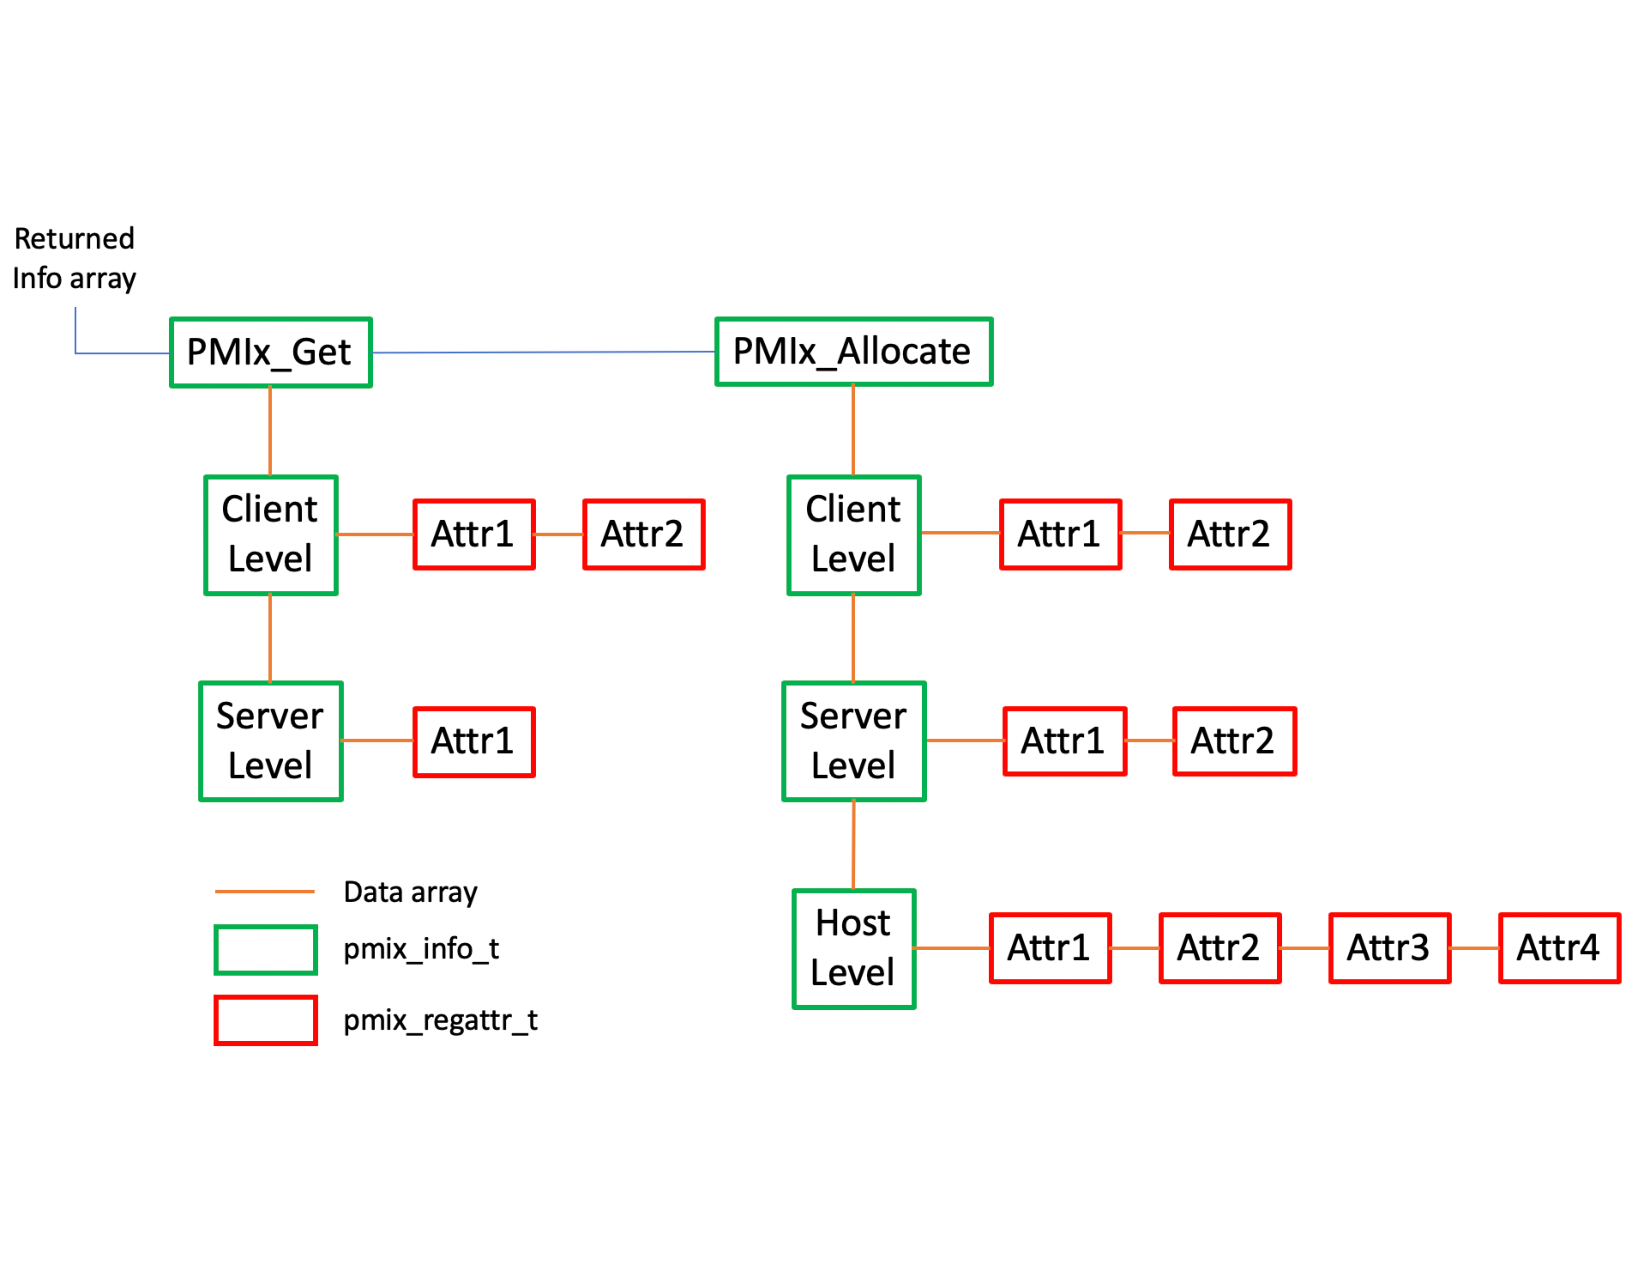
\includegraphics[clip,width=0.75\textwidth]{figs/attrquery.pdf}
  \end{center}
  \caption{Returned information hierarchy for attribute support request}
  \label{fig:attrquery}
\end{figure*}
\endgroup

The array of returned structures, and their child arrays, are subject to the return rules for the \refapi{PMIx_Query_info_nb} \ac{API}. For example, a request for supported attributes of the \refapi{PMIx_Get} function that includes the \refarg{host} level will return values for the \refarg{client} and \refarg{server} levels, plus an array element with a \refarg{key} of \refattr{PMIX_HOST_ATTRIBUTES} and a value type of \refconst{PMIX_UNDEF} indicating that no attributes are supported at that level.

%%%%%%%%%%%%%%%%%%%%%%%%%%%%%%%%%%%%%%%%%%%%%%
%%%%%%%%%%%%%%%%%%%%%%%%%%%%%%%%%%%%%%%%%%%%%%
\section{Allocation Requests}
\label{chap:api_job_mgmt:alloc}

This section defines functionality to request new allocations from the \ac{RM}, and request modifications to existing allocations.
These are primarily used in the following scenarios:
\begin{itemize}
\item \textit{Evolving} applications that dynamically request and return resources as they execute
\item \textit{Malleable} environments where the scheduler redirects resources away from executing applications for higher priority jobs or load balancing
\item \textit{Resilient} applications that need to request replacement resources in the face of failures
\item \textit{Rigid} jobs where the user has requested a static allocation of resources for a fixed period of time, but realizes that they underestimated their required time while executing
\end{itemize}
\ac{PMIx} attempts to address this range of use-cases with a flexible \ac{API}.

%%%%%%%%%%%
\subsection{\code{PMIx_Allocation_request}}
\declareapi{PMIx_Allocation_request}

%%%%
\summary

Request an allocation operation from the host resource manager.

%%%%
\format

\versionMarker{3.0}
\cspecificstart
\begin{codepar}
pmix_status_t
PMIx_Allocation_request(pmix_alloc_directive_t directive,
                        pmix_info_t info[], size_t ninfo);
\end{codepar}
\cspecificend

\begin{arglist}
\argin{directive}{Allocation directive (handle)}
\argin{info}{Array of \refstruct{pmix_info_t} structures (array of handles)}
\argin{ninfo}{Number of elements in the \refarg{info} array (integer)}
\end{arglist}

Returns one of the following:

\begin{itemize}
    \item \refconst{PMIX_SUCCESS}, indicating that the request was processed and returned \textit{success}
    \item a PMIx error constant indicating either an error in the input or that the request was refused
\end{itemize}

\reqattrstart
\ac{PMIx} libraries are not required to directly support any attributes for this function. However, any provided attributes must be passed to the host \ac{SMS} daemon for processing, and the \ac{PMIx} library is \textit{required} to add the \refPRIAttributeItem{PMIX_USERID} and the \refPRIAttributeItem{PMIX_GRPID} attributes of the client process making the request.

\divider

Host environments that implement support for this operation are required to support the following attributes:

\pasteAttributeItem{PMIX_ALLOC_ID}
\pasteAttributeItem{PMIX_ALLOC_NUM_NODES}
\pasteAttributeItem{PMIX_ALLOC_NUM_CPUS}
\pasteAttributeItem{PMIX_ALLOC_TIME}

\reqattrend

\optattrstart
The following attributes are optional for host environments that support this operation:

\pasteAttributeItem{PMIX_ALLOC_NODE_LIST}
\pasteAttributeItem{PMIX_ALLOC_NUM_CPU_LIST}
\pasteAttributeItem{PMIX_ALLOC_CPU_LIST}
\pasteAttributeItem{PMIX_ALLOC_MEM_SIZE}
\pasteAttributeItem{PMIX_ALLOC_NETWORK}
\pasteAttributeItem{PMIX_ALLOC_NETWORK_ID}
\pasteAttributeItem{PMIX_ALLOC_BANDWIDTH}
\pasteAttributeItem{PMIX_ALLOC_NETWORK_QOS}
\pasteAttributeItem{PMIX_ALLOC_NETWORK_TYPE}
\pasteAttributeItem{PMIX_ALLOC_NETWORK_PLANE}
\pasteAttributeItem{PMIX_ALLOC_NETWORK_ENDPTS}
\pasteAttributeItem{PMIX_ALLOC_NETWORK_ENDPTS_NODE}
\pasteAttributeItem{PMIX_ALLOC_NETWORK_SEC_KEY}

\optattrend

%%%%
\descr

Request an allocation operation from the host resource manager.
Several broad categories are envisioned, including the ability to:

\begin{compactitem}
%
\item Request allocation of additional resources, including memory, bandwidth, and compute.
This should be accomplished in a non-blocking manner so that the application can continue to progress while waiting for resources to become available.
Note that the new allocation will be disjoint from (i.e., not affiliated with) the allocation of the requestor - thus the termination of one allocation will not impact the other.
%
\item Extend the reservation on currently allocated resources, subject to scheduling availability and priorities.
This includes extending the time limit on current resources, and/or requesting additional resources be allocated to the requesting job.
Any additional allocated resources will be considered as part of the current allocation, and thus will be released at the same time.
%
\item Return no-longer-required resources to the scheduler.
This includes the ``loan'' of resources back to the scheduler with a promise to return them upon subsequent request.
\end{compactitem}

%%%%%%%%%%%
\subsection{\code{PMIx_Allocation_request_nb}}
\declareapi{PMIx_Allocation_request_nb}

%%%%
\summary

Request an allocation operation from the host resource manager.

%%%%
\format

\versionMarker{2.0}
\cspecificstart
\begin{codepar}
pmix_status_t
PMIx_Allocation_request_nb(pmix_alloc_directive_t directive,
                           pmix_info_t info[], size_t ninfo,
                           pmix_info_cbfunc_t cbfunc, void *cbdata);
\end{codepar}
\cspecificend

\begin{arglist}
\argin{directive}{Allocation directive (handle)}
\argin{info}{Array of \refstruct{pmix_info_t} structures (array of handles)}
\argin{ninfo}{Number of elements in the \refarg{info} array (integer)}
\argin{cbfunc}{Callback function \refapi{pmix_info_cbfunc_t} (function reference)}
\argin{cbdata}{Data to be passed to the callback function (memory reference)}
\end{arglist}

Returns one of the following:

\begin{itemize}
    \item \refconst{PMIX_SUCCESS}, indicating that the request is being processed by the host environment - result will be returned in the provided \refarg{cbfunc}. Note that the library must not invoke the callback function prior to returning from the \ac{API}.
    \item \refconst{PMIX_OPERATION_SUCCEEDED}, indicating that the request was immediately processed and returned \textit{success} - the \refarg{cbfunc} will \textit{not} be called
    \item a PMIx error constant indicating either an error in the input or that the request was immediately processed and failed - the \refarg{cbfunc} will \textit{not} be called
\end{itemize}

\reqattrstart
\ac{PMIx} libraries are not required to directly support any attributes for this function. However, any provided attributes must be passed to the host \ac{SMS} daemon for processing, and the \ac{PMIx} library is \textit{required} to add the \refPRIAttributeItem{PMIX_USERID} and the \refPRIAttributeItem{PMIX_GRPID} attributes of the client process making the request.

\divider

Host environments that implement support for this operation are required to support the following attributes:

\pasteAttributeItem{PMIX_ALLOC_ID}
\pasteAttributeItem{PMIX_ALLOC_NUM_NODES}
\pasteAttributeItem{PMIX_ALLOC_NUM_CPUS}
\pasteAttributeItem{PMIX_ALLOC_TIME}

\reqattrend

\optattrstart
The following attributes are optional for host environments that support this operation:

\pasteAttributeItem{PMIX_ALLOC_NODE_LIST}
\pasteAttributeItem{PMIX_ALLOC_NUM_CPU_LIST}
\pasteAttributeItem{PMIX_ALLOC_CPU_LIST}
\pasteAttributeItem{PMIX_ALLOC_MEM_SIZE}
\pasteAttributeItem{PMIX_ALLOC_NETWORK}
\pasteAttributeItem{PMIX_ALLOC_NETWORK_ID}
\pasteAttributeItem{PMIX_ALLOC_BANDWIDTH}
\pasteAttributeItem{PMIX_ALLOC_NETWORK_QOS}
\pasteAttributeItem{PMIX_ALLOC_NETWORK_TYPE}
\pasteAttributeItem{PMIX_ALLOC_NETWORK_PLANE}
\pasteAttributeItem{PMIX_ALLOC_NETWORK_ENDPTS}
\pasteAttributeItem{PMIX_ALLOC_NETWORK_ENDPTS_NODE}
\pasteAttributeItem{PMIX_ALLOC_NETWORK_SEC_KEY}

\optattrend

%%%%
\descr

Non-blocking form of the \refapi{PMIx_Allocation_request} \ac{API}.


%%%%%%%%%%%%%%%%%%%%%%%%%%%%%%%%%%%%%%%%%%%%%%
%%%%%%%%%%%%%%%%%%%%%%%%%%%%%%%%%%%%%%%%%%%%%%
\section{Job Control}
\label{chap:api_job_mgmt:jctrl}

This section defines \acp{API} that enable the application and host environment to coordinate the response to failures and other events.
This can include requesting termination of the entire job or a subset of processes within a job, but can
also be used in combination with other \ac{PMIx} capabilities (e.g., allocation support and event notification) for more nuanced responses. For example, an application notified of an incipient over-temperature condition on a node could use the \refapi{PMIx_Allocation_request_nb} interface to request replacement nodes while simultaneously using the \refapi{PMIx_Job_control_nb} interface to direct that a checkpoint event be delivered to all processes in the application. If replacement resources are not available, the application might use the \refapi{PMIx_Job_control_nb} interface to request that the job continue at a lower power setting, perhaps sufficient to avoid the over-temperature failure.

The job control \acp{API} can also be used by an application to register itself as available for preemption when operating in an environment such as a cloud or where incentives, financial or otherwise, are provided to jobs willing to be preempted. Registration can include attributes indicating how many resources are being offered for preemption (e.g., all or only some portion), whether the application will require time to prepare for preemption, etc. Jobs that
request a warning will receive an event notifying them of an impending preemption (possibly including information as to the resources that will be taken away, how much time the application will be given prior to being preempted, whether the preemption will be a suspension or full termination, etc.) so they have an opportunity to save
their work. Once the application is ready, it calls the provided event completion callback function to indicate that
the SMS is free to suspend or terminate it, and can include directives regarding any desired restart.

%%%%%%%%%%%
\subsection{\code{PMIx_Job_control}}
\declareapi{PMIx_Job_control}

%%%%
\summary

Request a job control action.

%%%%
\format

\versionMarker{3.0}
\cspecificstart
\begin{codepar}
pmix_status_t
PMIx_Job_control(const pmix_proc_t targets[], size_t ntargets,
                 const pmix_info_t directives[], size_t ndirs)
\end{codepar}
\cspecificend

\begin{arglist}
\argin{targets}{Array of proc structures (array of handles)}
\argin{ntargets}{Number of element in the \refarg{targets} array (integer)}
\argin{directives}{Array of info structures (array of handles)}
\argin{ndirs}{Number of element in the \refarg{directives} array (integer)}
\argin{cbfunc}{Callback function \refapi{pmix_info_cbfunc_t} (function reference)}
\argin{cbdata}{Data to be passed to the callback function (memory reference)}
\end{arglist}

Returns one of the following:

\begin{itemize}
    \item \refconst{PMIX_SUCCESS}, indicating that the request was processed by the host environment and returned \textit{success}
    \item a \ac{PMIx} error constant indicating either an error in the input or that the request was refused
\end{itemize}

\reqattrstart
\ac{PMIx} libraries are not required to directly support any attributes for this function. However, any provided attributes must be passed to the host \ac{SMS} daemon for processing, and the \ac{PMIx} library is \textit{required} to add the \refPRIAttributeItem{PMIX_USERID} and the \refPRIAttributeItem{PMIX_GRPID} attributes of the client process making the request.

\divider

Host environments that implement support for this operation are required to support the following attributes:

\pastePRRTEAttributeItem{PMIX_JOB_CTRL_ID}
\pastePRRTEAttributeItem{PMIX_JOB_CTRL_PAUSE}
\pastePRRTEAttributeItem{PMIX_JOB_CTRL_RESUME}
\pastePRRTEAttributeItem{PMIX_JOB_CTRL_KILL}
\pastePRRTEAttributeItem{PMIX_JOB_CTRL_SIGNAL}
\pastePRRTEAttributeItem{PMIX_JOB_CTRL_TERMINATE}
\pastePRRTEAttributeItem{PMIX_REGISTER_CLEANUP}
\pastePRRTEAttributeItem{PMIX_REGISTER_CLEANUP_DIR}
\pastePRRTEAttributeItem{PMIX_CLEANUP_RECURSIVE}
\pastePRRTEAttributeItem{PMIX_CLEANUP_EMPTY}
\pastePRRTEAttributeItem{PMIX_CLEANUP_IGNORE}
\pastePRRTEAttributeItem{PMIX_CLEANUP_LEAVE_TOPDIR}

\reqattrend

\optattrstart
The following attributes are optional for host environments that support this operation:

\pasteAttributeItem{PMIX_JOB_CTRL_CANCEL}
\pasteAttributeItem{PMIX_JOB_CTRL_RESTART}
\pasteAttributeItem{PMIX_JOB_CTRL_CHECKPOINT}
\pasteAttributeItem{PMIX_JOB_CTRL_CHECKPOINT_EVENT}
\pasteAttributeItem{PMIX_JOB_CTRL_CHECKPOINT_SIGNAL}
\pasteAttributeItem{PMIX_JOB_CTRL_CHECKPOINT_TIMEOUT}
\pasteAttributeItem{PMIX_JOB_CTRL_CHECKPOINT_METHOD}
\pasteAttributeItem{PMIX_JOB_CTRL_PROVISION}
\pasteAttributeItem{PMIX_JOB_CTRL_PROVISION_IMAGE}
\pasteAttributeItem{PMIX_JOB_CTRL_PREEMPTIBLE}

\optattrend

%%%%
\descr

Request a job control action.
The \refarg{targets} array identifies the processes to which the requested job control action is to be applied.
A \code{NULL} value can be used to indicate all processes in the caller's namespace.
The use of \refconst{PMIX_RANK_WILDCARD} can also be used to indicate that all processes in the given namespace are to be included.

The directives are provided as \refstruct{pmix_info_t} structures in the \refarg{directives} array.
The callback function provides a \refarg{status} to indicate whether or not the request was granted, and to provide some information as to the reason for any denial in the \refapi{pmix_info_cbfunc_t} array of \refstruct{pmix_info_t} structures.

%%%%%%%%%%%
\subsection{\code{PMIx_Job_control_nb}}
\declareapi{PMIx_Job_control_nb}

%%%%
\summary

Request a job control action.

%%%%
\format

\versionMarker{2.0}
\cspecificstart
\begin{codepar}
pmix_status_t
PMIx_Job_control_nb(const pmix_proc_t targets[], size_t ntargets,
                    const pmix_info_t directives[], size_t ndirs,
                    pmix_info_cbfunc_t cbfunc, void *cbdata)
\end{codepar}
\cspecificend

\begin{arglist}
\argin{targets}{Array of proc structures (array of handles)}
\argin{ntargets}{Number of element in the \refarg{targets} array (integer)}
\argin{directives}{Array of info structures (array of handles)}
\argin{ndirs}{Number of element in the \refarg{directives} array (integer)}
\argin{cbfunc}{Callback function \refapi{pmix_info_cbfunc_t} (function reference)}
\argin{cbdata}{Data to be passed to the callback function (memory reference)}
\end{arglist}

Returns one of the following:

\begin{itemize}
    \item \refconst{PMIX_SUCCESS}, indicating that the request is being processed by the host environment - result will be returned in the provided \refarg{cbfunc}. Note that the library must not invoke the callback function prior to returning from the \ac{API}.
    \item \refconst{PMIX_OPERATION_SUCCEEDED}, indicating that the request was immediately processed and returned \textit{success} - the \refarg{cbfunc} will \textit{not} be called
    \item a PMIx error constant indicating either an error in the input or that the request was immediately processed and failed - the \refarg{cbfunc} will \textit{not} be called
\end{itemize}

\reqattrstart
\ac{PMIx} libraries are not required to directly support any attributes for this function. However, any provided attributes must be passed to the host \ac{SMS} daemon for processing, and the \ac{PMIx} library is \textit{required} to add the \refPRIAttributeItem{PMIX_USERID} and the \refPRIAttributeItem{PMIX_GRPID} attributes of the client process making the request.

\divider

Host environments that implement support for this operation are required to support the following attributes:

\pastePRRTEAttributeItem{PMIX_JOB_CTRL_ID}
\pastePRRTEAttributeItem{PMIX_JOB_CTRL_PAUSE}
\pastePRRTEAttributeItem{PMIX_JOB_CTRL_RESUME}
\pastePRRTEAttributeItem{PMIX_JOB_CTRL_KILL}
\pastePRRTEAttributeItem{PMIX_JOB_CTRL_SIGNAL}
\pastePRRTEAttributeItem{PMIX_JOB_CTRL_TERMINATE}
\pastePRRTEAttributeItem{PMIX_REGISTER_CLEANUP}
\pastePRRTEAttributeItem{PMIX_REGISTER_CLEANUP_DIR}
\pastePRRTEAttributeItem{PMIX_CLEANUP_RECURSIVE}
\pastePRRTEAttributeItem{PMIX_CLEANUP_EMPTY}
\pastePRRTEAttributeItem{PMIX_CLEANUP_IGNORE}
\pastePRRTEAttributeItem{PMIX_CLEANUP_LEAVE_TOPDIR}

\reqattrend

\optattrstart
The following attributes are optional for host environments that support this operation:

\pasteAttributeItem{PMIX_JOB_CTRL_CANCEL}
\pasteAttributeItem{PMIX_JOB_CTRL_RESTART}
\pasteAttributeItem{PMIX_JOB_CTRL_CHECKPOINT}
\pasteAttributeItem{PMIX_JOB_CTRL_CHECKPOINT_EVENT}
\pasteAttributeItem{PMIX_JOB_CTRL_CHECKPOINT_SIGNAL}
\pasteAttributeItem{PMIX_JOB_CTRL_CHECKPOINT_TIMEOUT}
\pasteAttributeItem{PMIX_JOB_CTRL_CHECKPOINT_METHOD}
\pasteAttributeItem{PMIX_JOB_CTRL_PROVISION}
\pasteAttributeItem{PMIX_JOB_CTRL_PROVISION_IMAGE}
\pasteAttributeItem{PMIX_JOB_CTRL_PREEMPTIBLE}

\optattrend

%%%%
\descr

Non-blocking form of the \refapi{PMIx_Job_control} \ac{API}.
The \refarg{targets} array identifies the processes to which the requested job control action is to be applied.
A \code{NULL} value can be used to indicate all processes in the caller's namespace.
The use of \refconst{PMIX_RANK_WILDCARD} can also be used to indicate that all processes in the given namespace are to be included.

The directives are provided as \refstruct{pmix_info_t} structures in the \refarg{directives} array.
The callback function provides a \refarg{status} to indicate whether or not the request was granted, and to provide some information as to the reason for any denial in the \refapi{pmix_info_cbfunc_t} array of \refstruct{pmix_info_t} structures.



%%%%%%%%%%%%%%%%%%%%%%%%%%%%%%%%%%%%%%%%%%%%%%
%%%%%%%%%%%%%%%%%%%%%%%%%%%%%%%%%%%%%%%%%%%%%%
\section{Process and Job Monitoring}
\label{chap:api_job_mgmt:monitor}

In addition to external faults, a common problem encountered in \ac{HPC} applications is a failure to make
progress due to some internal conflict in the computation. These situations can
result in a significant waste of resources as the \ac{SMS} is unaware of the problem, and thus cannot terminate the
job. Various watchdog methods have been developed for detecting this situation, including requiring a periodic ``heartbeat''
from the application and monitoring a specified file for changes in size and/or modification time.

At the request of \ac{SMS} vendors and members, a monitoring support interface has been included in the PMIx v2 standard. The defined \ac{API} allows applications to request monitoring, directing what is to be monitored, the frequency of the associated check, whether or not the application is to be notified (via the event notification subsystem) of stall detection, and other characteristics of the operation. In addition, heartbeat and file monitoring methods have been included in the \ac{PRI} but are active only when requested.

%%%%%%%%%%%
\subsection{\code{PMIx_Process_monitor}}
\declareapi{PMIx_Process_monitor}

%%%%
\summary

Request that application processes be monitored.

%%%%
\format

\versionMarker{3.0}
\cspecificstart
\begin{codepar}
pmix_status_t
PMIx_Process_monitor(const pmix_info_t *monitor, pmix_status_t error,
                     const pmix_info_t directives[], size_t ndirs)
\end{codepar}
\cspecificend

\begin{arglist}
\argin{monitor}{info (handle)}
\argin{error}{status (integer)}
\argin{directives}{Array of info structures (array of handles)}
\argin{ndirs}{Number of elements in the \refarg{directives} array (integer)}
\end{arglist}

Returns one of the following:

\begin{itemize}
    \item \refconst{PMIX_SUCCESS}, indicating that the request was processed and returned \textit{success}
    \item a PMIx error constant indicating either an error in the input or that the request was refused
\end{itemize}

\optattrstart
The following attributes may be implemented by a \ac{PMIx} library or by the host environment. If supported by the \ac{PMIx} server library, then the library must not pass the supported attributes to the host environment. All attributes not directly supported by the server library must be passed to the host environment if it supports this operation, and the library is \textit{required} to add the \refPRIAttributeItem{PMIX_USERID} and the \refPRIAttributeItem{PMIX_GRPID} attributes of the requesting process:

\pastePRIAttributeItem{PMIX_MONITOR_ID}
\pastePRIAttributeItem{PMIX_MONITOR_CANCEL}
\pastePRIAttributeItem{PMIX_MONITOR_APP_CONTROL}
\pastePRIAttributeItem{PMIX_MONITOR_HEARTBEAT}
\pastePRIAttributeItem{PMIX_MONITOR_HEARTBEAT_TIME}
\pastePRIAttributeItem{PMIX_MONITOR_HEARTBEAT_DROPS}
\pastePRIAttributeItem{PMIX_MONITOR_FILE}
\pastePRIAttributeItem{PMIX_MONITOR_FILE_SIZE}
\pastePRIAttributeItem{PMIX_MONITOR_FILE_ACCESS}
\pastePRIAttributeItem{PMIX_MONITOR_FILE_MODIFY}
\pastePRIAttributeItem{PMIX_MONITOR_FILE_CHECK_TIME}
\pastePRIAttributeItem{PMIX_MONITOR_FILE_DROPS}

\optattrend

%%%%
\descr

Request that application processes be monitored via several possible methods.
For example, that the server monitor this process for periodic heartbeats as an indication that the process has not become ``wedged''.
When a monitor detects the specified alarm condition, it will generate an event notification using the provided error code and passing along any available relevant information.
It is up to the caller to register a corresponding event handler.

The \refarg{monitor} argument is an attribute indicating the type of monitor being requested.
For example, \refattr{PMIX_MONITOR_FILE} to indicate that the requestor is asking that a file be monitored.

The \refarg{error} argument is the status code to be used when generating an event notification alerting that the monitor has been triggered.
The range of the notification defaults to \refconst{PMIX_RANGE_NAMESPACE}.
This can be changed by providing a \refattr{PMIX_RANGE} directive.

The \refarg{directives} argument characterizes the monitoring request (e.g., monitor file size) and frequency of checking to be done


%%%%%%%%%%%
\subsection{\code{PMIx_Process_monitor_nb}}
\declareapi{PMIx_Process_monitor_nb}

%%%%
\summary

Request that application processes be monitored.

%%%%
\format

\versionMarker{2.0}
\cspecificstart
\begin{codepar}
pmix_status_t
PMIx_Process_monitor_nb(const pmix_info_t *monitor, pmix_status_t error,
                        const pmix_info_t directives[], size_t ndirs,
                        pmix_info_cbfunc_t cbfunc, void *cbdata)
\end{codepar}
\cspecificend

\begin{arglist}
\argin{monitor}{info (handle)}
\argin{error}{status (integer)}
\argin{directives}{Array of info structures (array of handles)}
\argin{ndirs}{Number of elements in the \refarg{directives} array (integer)}
\argin{cbfunc}{Callback function \refapi{pmix_info_cbfunc_t} (function reference)}
\argin{cbdata}{Data to be passed to the callback function (memory reference)}
\end{arglist}

Returns one of the following:

\begin{itemize}
    \item \refconst{PMIX_SUCCESS}, indicating that the request is being processed by the host environment - result will be returned in the provided \refarg{cbfunc}. Note that the library must not invoke the callback function prior to returning from the \ac{API}.
    \item \refconst{PMIX_OPERATION_SUCCEEDED}, indicating that the request was immediately processed and returned \textit{success} - the \refarg{cbfunc} will \textit{not} be called
    \item a PMIx error constant indicating either an error in the input or that the request was immediately processed and failed - the \refarg{cbfunc} will \textit{not} be called
\end{itemize}

\optattrstart
The following attributes may be implemented by a \ac{PMIx} library or by the host environment. If supported by the \ac{PMIx} server library, then the library must not pass the supported attributes to the host environment. All attributes not directly supported by the server library must be passed to the host environment if it supports this operation, and the library is \textit{required} to add the \refPRIAttributeItem{PMIX_USERID} and the \refPRIAttributeItem{PMIX_GRPID} attributes of the requesting process:

\pastePRIAttributeItem{PMIX_MONITOR_ID}
\pastePRIAttributeItem{PMIX_MONITOR_CANCEL}
\pastePRIAttributeItem{PMIX_MONITOR_APP_CONTROL}
\pastePRIAttributeItem{PMIX_MONITOR_HEARTBEAT}
\pastePRIAttributeItem{PMIX_MONITOR_HEARTBEAT_TIME}
\pastePRIAttributeItem{PMIX_MONITOR_HEARTBEAT_DROPS}
\pastePRIAttributeItem{PMIX_MONITOR_FILE}
\pastePRIAttributeItem{PMIX_MONITOR_FILE_SIZE}
\pastePRIAttributeItem{PMIX_MONITOR_FILE_ACCESS}
\pastePRIAttributeItem{PMIX_MONITOR_FILE_MODIFY}
\pastePRIAttributeItem{PMIX_MONITOR_FILE_CHECK_TIME}
\pastePRIAttributeItem{PMIX_MONITOR_FILE_DROPS}

\optattrend

%%%%
\descr


Non-blocking form of the \refapi{PMIx_Process_monitor} \ac{API}. The \refarg{cbfunc} function provides a \refarg{status} to indicate whether or not the request was granted, and to provide some information as to the reason for any denial in the \refapi{pmix_info_cbfunc_t} array of \refstruct{pmix_info_t} structures.

%%%%%%%%%%%
\subsection{\code{PMIx_Heartbeat}}
\declaremacro{PMIx_Heartbeat}

%%%%
\summary

Send a heartbeat to the \ac{PMIx} server library

%%%%
\format

\versionMarker{2.0}
\cspecificstart
\begin{codepar}
PMIx_Heartbeat(void)
\end{codepar}
\cspecificend


%%%%
\descr

A simplified macro wrapping \refapi{PMIx_Process_monitor_nb} that sends a heartbeat to the \ac{PMIx} server library.


%%%%%%%%%%%%%%%%%%%%%%%%%%%%%%%%%%%%%%%%%%%%%%
%%%%%%%%%%%%%%%%%%%%%%%%%%%%%%%%%%%%%%%%%%%%%%
\section{Logging}
\label{chap:api_job_mgmt:logging}

The logging interface supports posting information by applications and SMS elements to persistent storage. This function is \textit{not} intended for output of computational results, but rather for reporting status and saving state information such as inserting computation progress reports into the application's \ac{SMS} job log or error reports to the local syslog.

\subsection{\code{PMIx_Log}}
\declareapi{PMIx_Log}

%%%%
\summary

Log data to a data service.

%%%%
\format

\versionMarker{3.0}
\cspecificstart
\begin{codepar}
pmix_status_t
PMIx_Log(const pmix_info_t data[], size_t ndata,
         const pmix_info_t directives[], size_t ndirs)
\end{codepar}
\cspecificend

\begin{arglist}
\argin{data}{Array of info structures (array of handles)}
\argin{ndata}{Number of elements in the \refarg{data} array (\code{size_t})}
\argin{directives}{Array of info structures (array of handles)}
\argin{ndirs}{Number of elements in the \refarg{directives} array (\code{size_t})}
\end{arglist}

Return codes are one of the following:

\begin{constantdesc}
    \item \refconst{PMIX_SUCCESS} The logging request was successful.
    \item \refconst{PMIX_ERR_BAD_PARAM} The logging request contains at least one incorrect entry.
    \item \refconst{PMIX_ERR_NOT_SUPPORTED} The \ac{PMIx} implementation or host environment does not support this function.
\end{constantdesc}

\reqattrstart
If the \ac{PMIx} library does not itself perform this operation, then it is required to pass any attributes provided by the client to the host environment for processing. In addition, it must include the following attributes in the passed \refarg{info} array:

\pastePRIAttributeItem{PMIX_USERID}
\pastePRIAttributeItem{PMIX_GRPID}

\divider

Host environments or \ac{PMIx} libraries that implement support for this operation are required to support the following attributes:

\pastePRIAttributeItem{PMIX_LOG_STDERR}
\pastePRIAttributeItem{PMIX_LOG_STDOUT}
\pastePRIAttributeItem{PMIX_LOG_SYSLOG}
\pastePRIAttributeItem{PMIX_LOG_LOCAL_SYSLOG}
\pastePRIAttributeItem{PMIX_LOG_GLOBAL_SYSLOG}
\pastePRIAttributeItem{PMIX_LOG_SYSLOG_PRI}
\pastePRIAttributeItem{PMIX_LOG_ONCE}

\reqattrend

\optattrstart
The following attributes are optional for host environments or \ac{PMIx} libraries that support this operation:

\pastePRIAttributeItem{PMIX_LOG_SOURCE}
\pastePRIAttributeItem{PMIX_LOG_TIMESTAMP}
\pastePRIAttributeItem{PMIX_LOG_GENERATE_TIMESTAMP}
\pastePRIAttributeItem{PMIX_LOG_TAG_OUTPUT}
\pastePRIAttributeItem{PMIX_LOG_TIMESTAMP_OUTPUT}
\pastePRIAttributeItem{PMIX_LOG_XML_OUTPUT}
\pastePRRTEAttributeItem{PMIX_LOG_EMAIL}
\pastePRRTEAttributeItem{PMIX_LOG_EMAIL_ADDR}
\pastePRRTEAttributeItem{PMIX_LOG_EMAIL_SUBJECT}
\pastePRRTEAttributeItem{PMIX_LOG_EMAIL_MSG}
\pasteAttributeItem{PMIX_LOG_JOB_RECORD}
\pasteAttributeItem{PMIX_LOG_GLOBAL_DATASTORE}

\optattrend

%%%%
\descr

Log data subject to the services offered by the host environment. The data to be logged is provided in the \refarg{data} array. The (optional) \refarg{directives} can be used to direct the choice of logging channel.

\adviceuserstart
It is strongly recommended that the \refapi{PMIx_Log} API not be used by applications for streaming data as it is not a ``performant'' transport and can perturb the application since it involves the local \ac{PMIx} server and host \ac{SMS} daemon. Note that a return of \refconst{PMIX_SUCCESS} only denotes that the data was successfully handed to the appropriate system call (for local channels) or the host environment and does not indicate receipt at the final destination.
\adviceuserend

%
\subsection{\code{PMIx_Log_nb}}
\declareapi{PMIx_Log_nb}

%%%%
\summary

Log data to a data service.

%%%%
\format

\versionMarker{2.0}
\cspecificstart
\begin{codepar}
pmix_status_t
PMIx_Log_nb(const pmix_info_t data[], size_t ndata,
            const pmix_info_t directives[], size_t ndirs,
            pmix_op_cbfunc_t cbfunc, void *cbdata)
\end{codepar}
\cspecificend

\begin{arglist}
\argin{data}{Array of info structures (array of handles)}
\argin{ndata}{Number of elements in the \refarg{data} array (\code{size_t})}
\argin{directives}{Array of info structures (array of handles)}
\argin{ndirs}{Number of elements in the \refarg{directives} array (\code{size_t})}
\argin{cbfunc}{Callback function \refapi{pmix_op_cbfunc_t} (function reference)}
\argin{cbdata}{Data to be passed to the callback function (memory reference)}
\end{arglist}

Return codes are one of the following:

\begin{constantdesc}
\item \refconst{PMIX_SUCCESS} The logging request is valid and is being processed. The resulting status from the operation will be provided in the callback function. Note that the library must not invoke the callback function prior to returning from the \ac{API}.
\item \refconst{PMIX_OPERATION_SUCCEEDED}, indicating that the request was immediately processed and returned \textit{success} - the \refarg{cbfunc} will \textit{not} be called
\item \refconst{PMIX_ERR_BAD_PARAM} The logging request contains at least one incorrect entry that prevents it from being processed. The callback function will not be called.
\item \refconst{PMIX_ERR_NOT_SUPPORTED} The \ac{PMIx} implementation does not support this function. The callback function will not be called.
\end{constantdesc}

\reqattrstart
If the \ac{PMIx} library does not itself perform this operation, then it is required to pass any attributes provided by the client to the host environment for processing. In addition, it must include the following attributes in the passed \refarg{info} array:

\pastePRIAttributeItem{PMIX_USERID}
\pastePRIAttributeItem{PMIX_GRPID}

\divider

Host environments or \ac{PMIx} libraries that implement support for this operation are required to support the following attributes:

\pastePRIAttributeItem{PMIX_LOG_STDERR}
\pastePRIAttributeItem{PMIX_LOG_STDOUT}
\pastePRIAttributeItem{PMIX_LOG_SYSLOG}
\pastePRIAttributeItem{PMIX_LOG_LOCAL_SYSLOG}
\pastePRIAttributeItem{PMIX_LOG_GLOBAL_SYSLOG}
\pastePRIAttributeItem{PMIX_LOG_SYSLOG_PRI}
\pastePRIAttributeItem{PMIX_LOG_ONCE}

\reqattrend

\optattrstart
The following attributes are optional for host environments or \ac{PMIx} libraries that support this operation:

\pastePRIAttributeItem{PMIX_LOG_SOURCE}
\pastePRIAttributeItem{PMIX_LOG_TIMESTAMP}
\pastePRIAttributeItem{PMIX_LOG_GENERATE_TIMESTAMP}
\pastePRIAttributeItem{PMIX_LOG_TAG_OUTPUT}
\pastePRIAttributeItem{PMIX_LOG_TIMESTAMP_OUTPUT}
\pastePRIAttributeItem{PMIX_LOG_XML_OUTPUT}
\pastePRRTEAttributeItem{PMIX_LOG_EMAIL}
\pastePRRTEAttributeItem{PMIX_LOG_EMAIL_ADDR}
\pastePRRTEAttributeItem{PMIX_LOG_EMAIL_SUBJECT}
\pastePRRTEAttributeItem{PMIX_LOG_EMAIL_MSG}
\pasteAttributeItem{PMIX_LOG_JOB_RECORD}
\pasteAttributeItem{PMIX_LOG_GLOBAL_DATASTORE}

\optattrend

%%%%
\descr

Log data subject to the services offered by the host environment. The data to be logged is provided in the \refarg{data} array. The (optional) \refarg{directives} can be used to direct the choice of logging channel.
The callback function will be executed when the log operation has been completed. The \refarg{data} and \refarg{directives} arrays must be maintained until the callback is provided.

\adviceuserstart
It is strongly recommended that the \refapi{PMIx_Log_nb} API not be used by applications for streaming data as it is not a ``performant'' transport and can perturb the application since it involves the local \ac{PMIx} server and host \ac{SMS} daemon. Note that a return of \refconst{PMIX_SUCCESS} only denotes that the data was successfully handed to the appropriate system call (for local channels) or the host environment and does not indicate receipt at the final destination.
\adviceuserend

%%%%%%%%%%%%%%%%%%%%%%%%%%%%%%%%%%%%%%%%%%%%%%%%%
